\documentclass{article}
\usepackage{amsmath}
\usepackage{float}
\usepackage{graphicx}
\author{Xin Gao, ID: 22984425}
\title{Enceladus: A Hidden World}
\begin{document}
\maketitle
\section{Introduction}
Enceladus is an icy world orbiting Saturn and, from recent observations,
may be a new frontier for space exploration and astrophysical
research. It is a relatively small moon with a cross sectional size of
England's area. Despite its small size, it is uniquely interesting as
the first body discovered to have ice jets shooting from geyser-like
openings. Does Enceladus in fact have a subsurface ocean and one that is
capable of hosting life? Based on direct observations and numerical
analyses, it is very likely that Enceladus have a reservoir of liquid
water beneath its icy crust.
\section{The South Polar Region}
Very little was known about Enceladus until 2005, when the
Cassini-Huygens spacecraft imaged details of Enceladus' surface for the
first time. Enceladus featured a region, later to be known as the 'tiger
stripes,' in the southern hemisphere where water ice jets seem to be
erupting from. Whereas most of Enceladus' surface is composed of
granular fine ice, the site of the cryovolcanic activities are primarily
composed of crystalline ice due to geological activity and higher
temperature. The south polar region is also the location of a detected
hemisphere, which formed from the material ejected by the jets. Analyses
concluded that the atmosphere is composed of approximately 91 percent
water vapor and is a major source of Saturn's E Ring. The peculiarities
of these region indicates a differentiated body and the existence of a
subsurface ocean inside the southern hemisphere. 
\section{Cryovolcanism and Internal Mechanisms}
The observed cryovolcanic activities are indicative of an active
interior. A form is heating mechanicsm would most likely be necessary to
maintain a subsurface liquid water ocean, if such an ocean is indeed
responsible for the ice jets.
\begin{figure}[h]
\centering
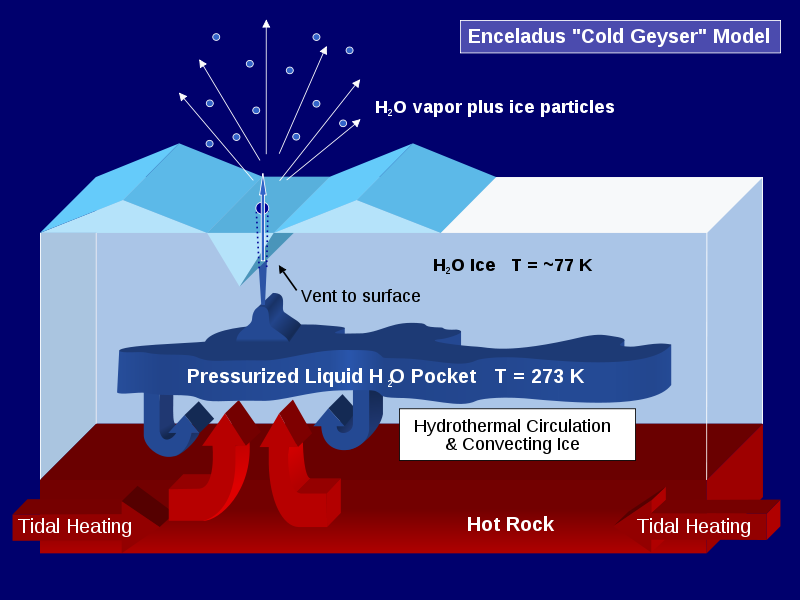
\includegraphics[width=.7\textwidth]{enceladus_heating.png}
\caption{A schematic drawing of the possible underlying mechanisms in
  the interior of Enceladus. Tidal heating support a dynamic magma
  mantle which provides thermal circulation for a layer of liquid water
  ocean above and the resulting cryovolcanism. 
  Source: wikipedia.org/wiki/Enceladus}
\end{figure}
Tidal heating can easily be present to provide the necessary energy
source that would support the ocean. Tidal forces on Enceladus arise
from its interaction with nearby bodies such as Saturn and Dione. The
thermal energy from the tidal forces can differentiate the interior by
heating up the mantle, creating a bed of magma. Such an active interior
generate energy circulation upwards towards the surface. Between the
water ice crush and the magma mantle would be a layer in which
temperatures and conditions would favor the existence of a liquid water
ocean. This active ocean would in turn release energy through cracks in
the form of the observed cryovolcanic activities, releasing water ice
among other substances. Organic compounds such as methane, propane,
acetylene, and other hydrocarbons have been detected near areas with
cryovolcanic activity.
\section{Gravitational Data and Analysis}
Recent gravitational data analysis further supports the theory of the
subsurfance liquid water ocean. The Cassini-Huygens spacecraft returned
values of the gravitational force acting on it during it recent
Enceladus flybys. The spacecraft measured gravitational perturbations that
arise from irregularities within Enceladus. Gravitational Doppler
Effects induce a slightly perturbed velocity of the spacecraft and this
change in velocity can be measured as radio signals from instruments on
Earth. The effect can be measured with great precision - the effected
velocity is small as 90 micrometers per second. From observations of a
surface depression in the south polar region, there would be an expected
gravitational anomaly in measurements. The measured values corresponding
to the anomaly are not as relatively negative, compared to the rest of
Enceladus, as would be expected of an uniformly dense interior. The
gravitational potential of a body is:
\begin{align}V = \frac{GM}{r}[1-\sum\limits_{l=1}^\infty
  J_{2l}\big[\frac{a}{r}\big]^{2l}P_{2l}cos(\theta)] 
\end{align}
where $P_{2l}cos(\theta)$ are the Legendre polynomials and
$J_{2l}\big[\frac{a}{r}\big]^{2l}$ are the gravitational moments of
inertia. The general form of the potential, as derived as the solution
to Laplace's Equation, is:
\begin{align}V = \frac{1}{a}[\sum\limits_{l=1}^\infty\sum\limits_{m=0}^l 
  \big[\frac{a}{r}\big]^{l+1}(C_{lm}cos(m\phi) +
  S_{lm}sin(m\phi))P_{l}^{m}cos(\theta)] 
\end{align}
where C and S are coefficients of the spherical harmonics and $\phi$ is
the azimuthal angle denoting longitude. A ratio of $\frac{J_{2}}{C_{22}}
= 3$ would indicate a body in hydrostatic equilibrium. The measured
value of this ratio is around 3.51, which is indicative of a
differentiated body. The interior of the southern hemisphere is
therefore extrapolated to be approximately seven percent more dense than
the surface ice. The existence of a hidden liquid water ocean in the
southern hemisphere would fill the gaps of the data analyses; it is in
correspondance with the values derived with the gravitational analysis
and with the measured Doppler Effects. 
\section{Conclusion}
Enceladus is looking quite promising as a frontier worth exploring. Due
to observations and the aforementioned data analyses, it is highly
likely that a stable liquid ocean water exists beneath the surface. The
possibility of it as a host for life is also realistic since, as far as
we know, there are no significant barriers from preventing it from
maintaining the conditions to do so. Enceladus is a world filled with
possibilities and more is to be known about it with planned future
flybys and possibly even probe missions.

\newpage

Brown, Dwayne; Platt, Jane; Bell, Brian. 'NASA Space Assets Detect Ocean
Inside Saturn Moon.' 3 April
2014. www.nasa.gov/press/2014/april/nasa-space-assets-detect-ocean-inside-saturn-moon/\#.USJEKjkSRux

Iess, L. et al. 'The Gravity Field and Interior of Enceladus.' 4 April
2014. \textit{Science}. www.sciencemag.org

Stevenson's Notes. Chapter 12: 'The Gravity Field and Gravitational Response to Rotation.'

'Enceladus.' Last accessed: 1 May 2014. wikipedia.org/wiki/Enceladus. 
\end{document}